\pagestyle{empty}
\cleardoublepage
\pagestyle{fancy}

\chapter{Modelagem Dinâmica} \label{Cap:Modelagem:Dinamica}

 Nesse capítulo abordaremos a modelagem dinâmica do rotor que sofre influências das forças do estator externo e dos polos do estator interno. Um modelo linearizado no ponto de operação é apresentando.
 
%Passos da modelagem:
%
%\begin{enumerate}[a.]
%	\item Imãs
%	\item Enrolamento
%	\item Rotor
%	\item Equação
%	\item Linearização
%\end{enumerate}



\section{Rotor}

A dinâmica do rotor é levantada a partir das forças resultantes aplicadas no rotor, essas forças são devido tanto aos imãs permanentes quanto pela força gerada pelas bobinas. A Fig. \ref{fig:modelo:forcas} ilustra as forças atuantes no rotor, onde :

 \begin{itemize}
 	\item $F_p$ : Força devido ao imã permanente
 	\item $F_b$ : Força devido a bobina
 	\item $\tau$ : Torque de rotação devido ao motor
 	\item $\theta$ : O angulo do rotor
 	\item $x,y,z$ : Deslocamento no plano cartesiano 
 \end{itemize}

 \begin{figure}[th]
 	\centering
 	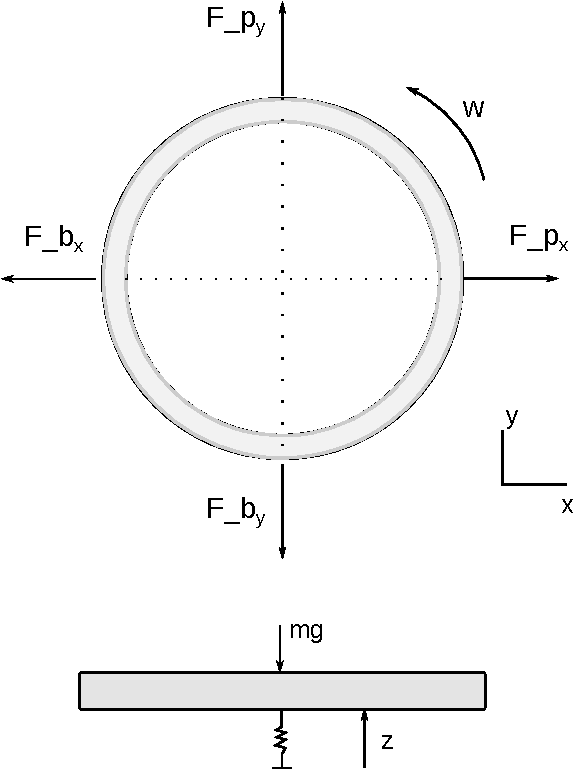
\includegraphics[width=0.5\linewidth]{../Figs/Modelagem/forcas}
 	\caption{Forças resultantes no rotor}
 	\label{fig:modelo:forcas}
 \end{figure}
 
 Via formalismo lagrangiano obtemos a parcela da energia cinética que é resultante da rotação, e das translações do rotor:
 
 \begin{align}
 	T_{\theta, x, y, z} &= \frac{1}{2} I_z \, \dot{\theta}^2 + \frac{1}{2} \, m \, \left( \dot{x}^2 + \dot{y}^2 + \dot{z}^2 \right) \notag \\
 \end{align}
 
 A energia potencial devido a translação axial do rotor:
 
 \begin{eqnarray}
 	V_z = m \, g \, z + \frac{1}{2} \, K \, z^2
 \end{eqnarray}
 
As forças não conservativas atuantes no rotor são causadas pela parte ativa do mancal:
 
 \begin{align}
 	Q_y^{nc} &= F_{by}(x,y,i)  \\
 	Q_x^{nc} &= F_{bx}(x,y,i)  
 \end{align}
 
As forças conservativas  (que dependem somente da posição do rotor) são resultantes dos imãs permanentes no estator externo :
 
 \begin{align}
 	Q_y^{c} &= F_{py}(x)  \\
 	Q_x^{c} &= F_{px}(y)  \\
 	Q_z^{c} &= F_{pz}(z)
 \end{align}
 
 Com a resolução da lagrangiana obtemos as equações da dinâmica do sistema:
  
 \begin{align}
 		L = T - V \notag \\
 		\frac{\partial}{\partial t} \left[ \frac{\partial L}{\partial \dot{r}} \right] -  \frac{\partial L}{\partial r} = Q^{nc} + Q^{c}
 \end{align}
 
Obtemos as equações diferencias que regem o modelo:
 
 \begin{align}
	I \ddot{\theta} &= 0 \\
	m \ddot{x}		&=  F_{px}(x,y) - F_{by}(x,y,i) \\
	m \ddot{y}		&=  F_{py}(x,y) - F_{bx}(x,y,i)\\	
	m \ddot{z} - K z &= m g  + F_{pz}
 \end{align}
 
 Exceto pela dependência das posições nas forças, verificamos pelas equações o desacoplamento entre os diferentes graus de liberdade. 
 
 
%\section{Rotor}
%
%Como não há acoplamento entre os eixos x,y e Z, A dinâmica do rotor é regida 


\section{Estator externo}

A força exercida no rotor devido aos imãs permanentes do estator externo podem ser aproximadas por uma equação linear, como visto em \ref{subsection:forca:x}. Assumisse que a força de atração no roto para pequenos deslocamento dependa somente da posição no eixo, podendo ser representada pela decomposição:

\begin{align}
	F_p(x) &= K_p \, x \\
	F_p(y) &= K_p \, y 
\end{align}

Onde $K_p$ é a constante de proporção entre a força e a posição, x e y são os deslocamento em torno do ponto de equilibro do rotor com relação ao estator externo. Obtemos via a simulação em elementos finitos um relação força por deslocamento de: $ F_p(d) = 547.8 \,d $ (distância em mm) para ambos os eixos (devido a simetria do mancal).

\section{Estator interno}

A força de atração do rotor devido ao campo magnético gerado pelas bobinas é não linear com a posição do rotor (comprimento do entreferro) e depende da corrente de excitação aplicada as bobinas. Além desses fatores, uma dinâmica do atuador atrelada a indutância deve ser considerada. A bobina é modelada como um circuito RL, como demonstrado na Fig. \ref{fig:dinamico:EI:Bobina}.

\begin{figure}[th!]
\centering
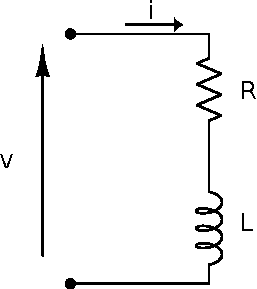
\includegraphics[width=0.2\linewidth]{Figs/Modelagem/EI_Bobina}
\caption{}
\label{fig:dinamico:EI:Bobina}
\end{figure}

\begin{align}
	I(s) &= \frac{V(s)}{R + L \, s} 
\end{align}

As indutâncias devem ser calculadas como demonstrada na SubSec. \ref{subsec:at:indutancia}. Os valores nominais (ponto de operação) da indutância de cada bobina é de aproximadamente 56mH e a resistência elétrica de 4 $\Omega$ gerando uma frequência de corte de 11 Hz. A força exercida por cada bobina é calculada pela forma analisada em: \eqref{eq:ativo:F:resultante:y}.

%\ref{fig:blocos:tensao:bobinas:x:y}.
%\begin{figure}[th]
%\centering
%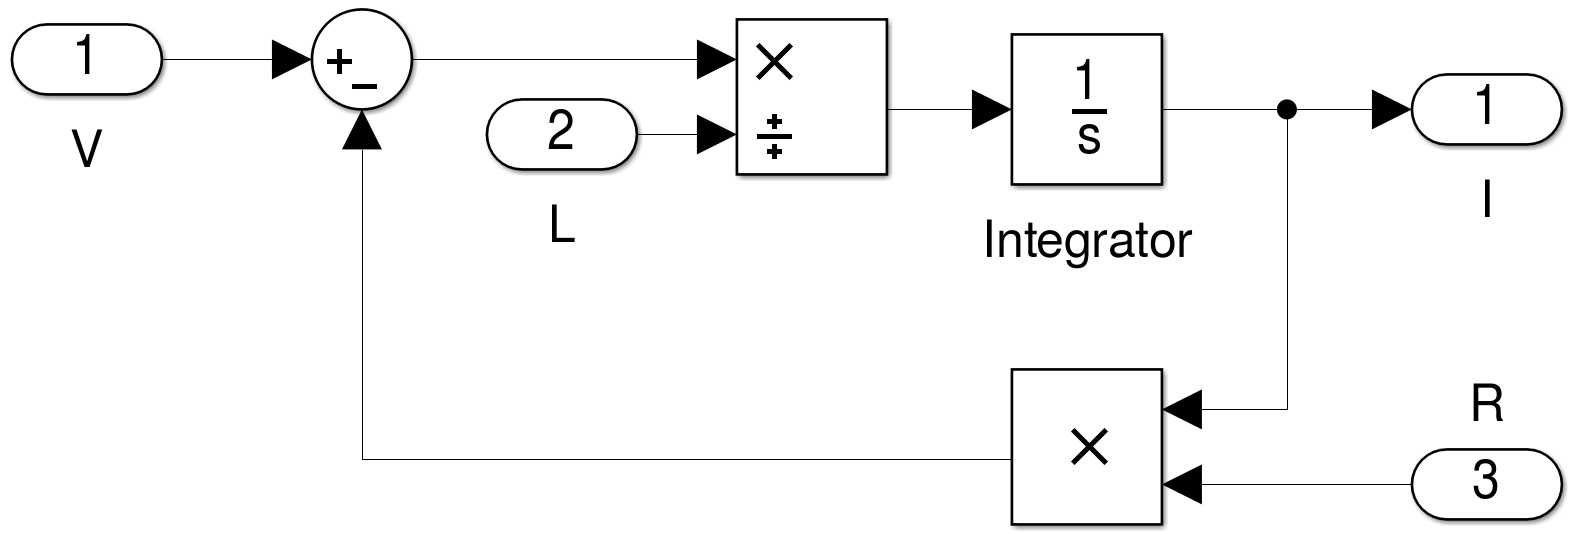
\includegraphics[width=0.7\linewidth]{./Figs/Modelagem/tensao-corrente-bobina}
%\caption{Diagrama de blocos bobina - Circuito ativo}
%\label{fig:tensao-corrente-bobina}
%\end{figure}

As tensões nas bobinas são distribuídas conforme Fig. \ref{fig:blocos:tensao:bobinas:x:y} (a), onde existe sobreposição de bobinas para atuação em diferentes eixos (X e Y). É aplicado nas bobinas que possuem sobreposição a metade da tensão, limitando assim o valor da tensão total nas bobinas para o valor máximo (I/2 + I/2 = I). A Fig. \ref{fig:blocos:tensao:bobinas:x:y} ilustra a configuração proposta. Verificamos que a tensão é aplicada em metade para as bobinas com sobreposição (a,g,e,c) e com ganho unitário nas bobinas principais (h,f,c,b). O Valor da indutância L varia em cada bobina pois depende do tamanho do entreferro.

%A força é então calculada por (a sua direção depende das bobinas acionadas) :

\begin{figure}[th]
\centering
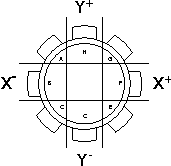
\includegraphics[width=0.5\linewidth]{./Figs/Modelagem/ativo-atuadores-conexao}
%
%\subfloat[Ganho das tensões nas bobinas]{
%\includegraphics[height=0.8\textheight]{./Figs/Modelagem/tensao:bobinas:x:y}}
%%
\caption{Distribuição das tensões nas bobinas}
\label{fig:blocos:tensao:bobinas:x:y}
\end{figure}

\subsection{Linearização da força}

Foi levantando em elementos finitos as forças magnéticas dado uma variação de posição (a partir do ponto de operação) de até 0.3mm e uma variação de corrente de 0A até 1A, um polinômio de primeiro grau foi encontrado com os resultados das forças. Optou-se trabalhar no ponto de corrente perto do zero pois é a região natural de operação dos polos. E com o rotor em torno do ponto de operação. O ganho para o sistema nessas condições é :
\begin{equation}
     F_b(i) = i \,    46.5383 
\end{equation}

\section{Batente}

O batente atua como uma saturação na posição do rotor (x,y), porém atrelou-se uma dinâmica ao batente para analisar as influências de possíveis choques mecânicos do rotor. Utilizou-se no  modelo o módulo de elasticidade (módulo de Young), onde a penetração ($\Delta l $) no material pode ser calculada por :

\begin{equation}
	\Delta l =  \frac{F l_o}{E \, A}
\end{equation}

Sendo : \textbf{E }a constante de Yong para o material; \textbf{A} área de contato; \textbf{$l_o$ } o comprimento inicial do material e \textbf{F} a força resultante do impacto. 

\section{Característica do sistema e diagrama de blocos}

A partir do diagrama de blocos ilustrado na Fig. \ref{fig:diagrama:blocos:modelo:linear}, um modelo em torno do ponto de operação pode ser levantando, o modelo servirá para o projeto do controlador. O sistema é do tipo 0 possuindo três polos localizados em:  $[1.21 -1.21 -0.07] \, 10^ 3$, sua função de transferência é:

\begin{equation}
G(s) = \frac{46530}{ 0.02077 \, s^3 + 1.478 \, s^2 - 3.08e04 \,s - 2.191e06}
\end{equation}

\begin{figure}[th!]
\centering
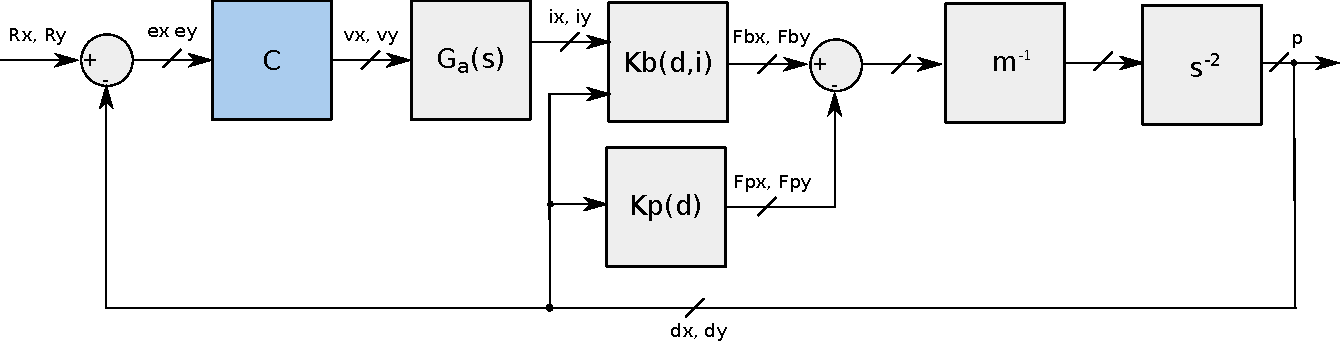
\includegraphics[width=1\linewidth]{../Figs/Modelagem/diagrama_blocos_modelo_linear}
\caption{Diagrama de blocos do modelo linearizado para descolamentos em x e y}
\label{fig:diagrama:blocos:modelo:linear}
\end{figure}

Verificamos através da analise em frequência (Fig. \ref{fig:bode:rlocus:pnt:operacao}) que o sistema é instável em malha aberta e um controlador deve ser projetado para instabilizar o sistema.	

\begin{figure}[th!]
\centering
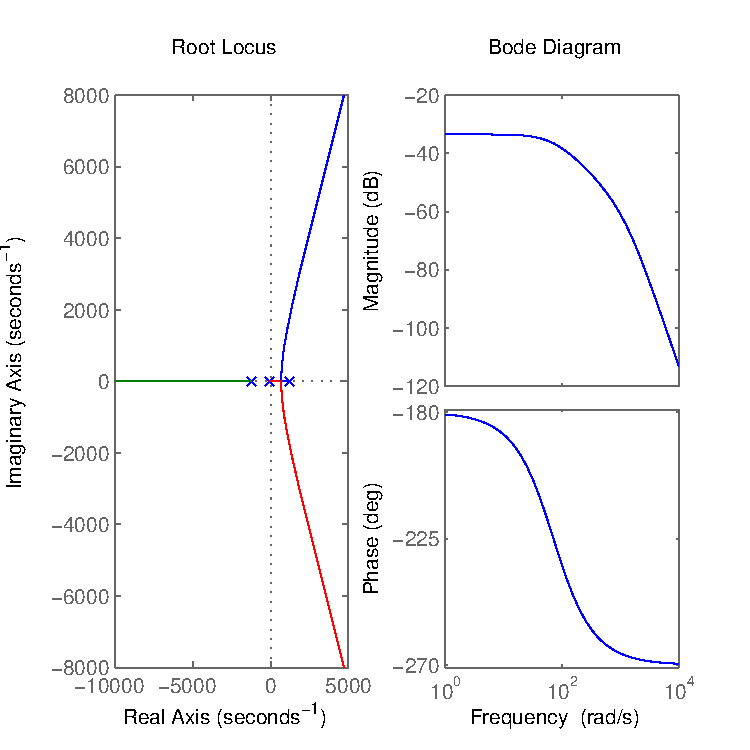
\includegraphics[width=0.7\linewidth]{./Figs/Modelagem/bode_rlocus_pnt_operacao}
\caption{Característica do sistema para um dos eixos em malha aberta}
\label{fig:bode:rlocus:pnt:operacao}
\end{figure}

\section{Simulações}

Simulações foram realizadas em malha aberta com o modelo não linear das forças,  a Fig. \ref{fig:dinamica:choque:rotor} é o comportamento do rotor quando nenhuma corrente é aplicada nos polos, verificamos  o choque com o batente em torno do 5ms.

\begin{figure}[th!]
\centering
\caption*{Posição x,y (mm) do rotor ao longo do tempo (s)}
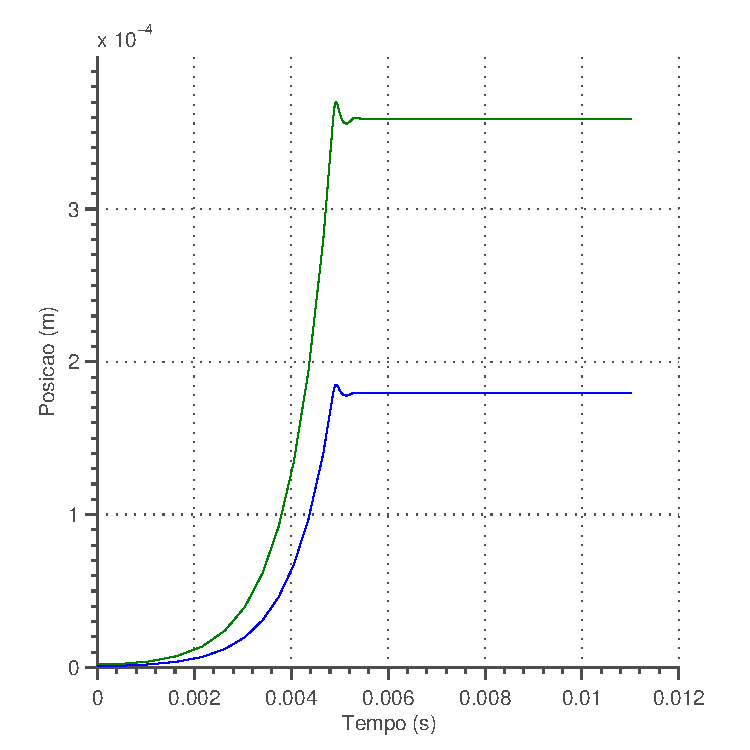
\includegraphics[width=0.7\linewidth]{./Modelagem/dinamica_choque_rotor}
\caption{Dinâmica instável do rotor e choque no batente}
\label{fig:dinamica:choque:rotor}
\end{figure}

A Fig. \ref{fig:dinamica:corrente:rotor} mostra o deslocamento do rotor dado a aplicação de 2.5 V nas bobinas x+,  verificamos a dinâmica da corrente dado a aplicação da corrente.

\begin{figure}[th!]
\centering
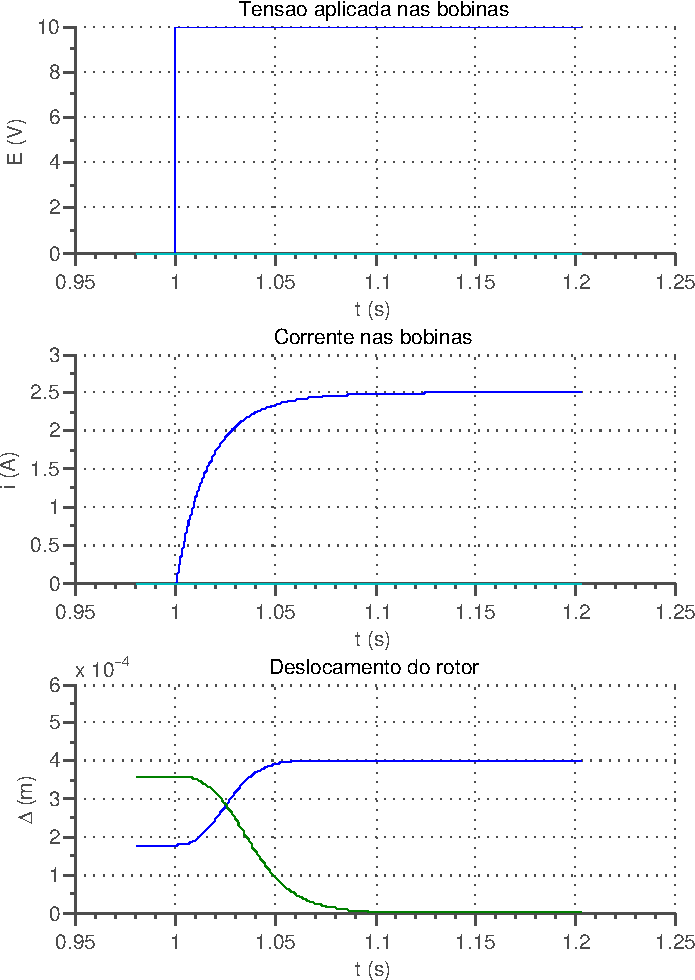
\includegraphics[width=0.7\linewidth]{./Modelagem/dinamica_corrente_rotor.pdf}
\caption{Dinâmica do rotor dado a aplicação de tensão na bobina X+}
\label{fig:dinamica:corrente:rotor}
\end{figure}

